\section{Elements\index{Elements}}

The base for every finite element computation is its mesh and the elements that are used within that mesh. What kind of element types can be used depends on the mesh, but also on the dimensionality of the problem (1D, 2D or 3D). In \akantu several isoparametric Langrangian element types are supported. Each of these types is discussed in some detail below, starting with the 1D-elements all the way to the 3D-elements. More detailed information (shape function, location of Gaussian quadrature points, and so on) can be found in Appendix~\ref{app:elements}. 

%%%%%%%%%% 1D %%%%%%%%%
\subsection{Isoparametric Elements in 1D\index{Elements!1D}}

In \akantu there are two types of isoparametric elements defined in 1D. These element types are called \code{segment\_2} and \code{segment\_3} and are depicted schematically in Figure~\ref{fig:elements:1D}. Some of the basic properties of these elements are listed in Table~\ref{tab:elements:1D}.

\begin{figure}[!htb]
\begin{center}
\begin{tabular}{m{0.3\textwidth}m{0.1\textwidth}m{0.3\textwidth}}
\subfloat[\code{segment\_2}]{
  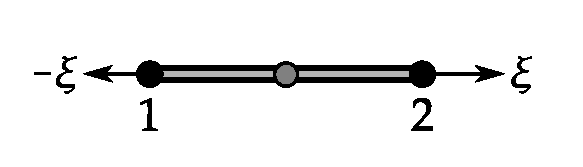
\includegraphics[width=0.3\textwidth]{figures/elements/segment_2}
  \label{fig:elements:segment2}
} & &
\subfloat[\code{segment\_3}]{
  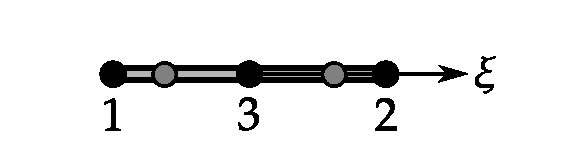
\includegraphics[width=0.3\textwidth]{figures/elements/segment_3}
  \label{fig:elements:segment3}
} 
\end{tabular}
\end{center}
\caption{A schematic overview of the three supported 1D element types in \akantu. In each element the node numbering as used in \akantu is indicated and also the quadrature points are highlighted (gray circles).}
\label{fig:elements:1D}
\end{figure}

\begin{table}[!htb]
\begin{center}
\begin{tabular}{l||c|c|c}
Element type & Order & \# nodes & \# quad. points \\
\hline
\code{segment\_2} & linear & 2 & 1 \\
\code{segment\_3} & quadratic & 3 & 2 \\
\end{tabular}
\end{center}
\caption{Some basic properties of the two 1D isoparametric elements in \akantu.}
\label{tab:elements:1D}
\end{table}

%%%%%%%%%% 2D %%%%%%%%%
\subsection{Isoparametric Elements in 2D\index{Elements!2D}}

In \akantu there are four types of isoparametric elements defined in 2D. These element types are called \code{triangle\_3}, \code{triangle\_6}, \code{quadrangle\_4} and \code{quadrangle\_8} and all of them are depicted in Figure~\ref{fig:elements:2D}. As with the 1D elements some of the most basic properties of these elements are listed in Table~\ref{tab:elements:2D}.

\begin{figure}[!htb]
\begin{center}
\begin{tabular}{m{0.3\textwidth}m{0.1\textwidth}m{0.3\textwidth}}
\subfloat[\code{triangle\_3}]{
  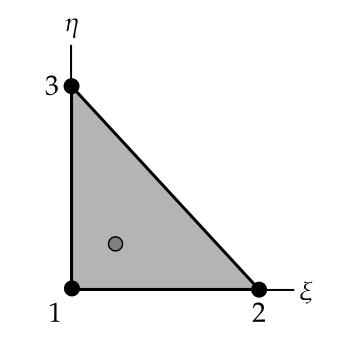
\includegraphics[width=0.3\textwidth]{figures/elements/triangle_3}
  \label{fig:elements:triangle3}
} & &
\subfloat[\code{triangle\_6}]{
  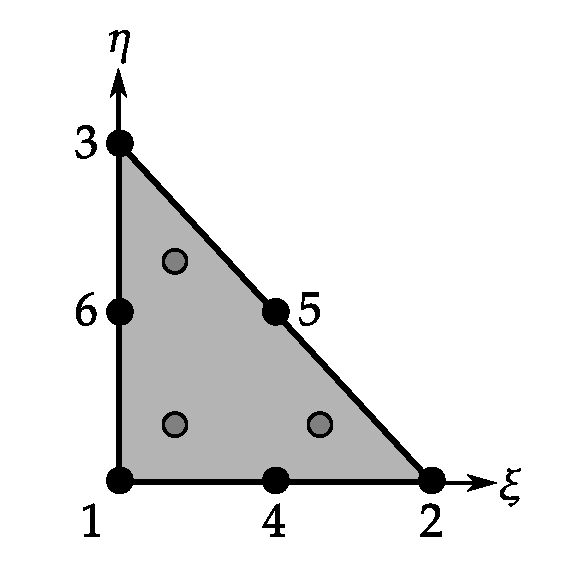
\includegraphics[width=0.3\textwidth]{figures/elements/triangle_6}
  \label{fig:elements:triangle6}
} \\
\subfloat[\code{quadrangle\_4}]{
  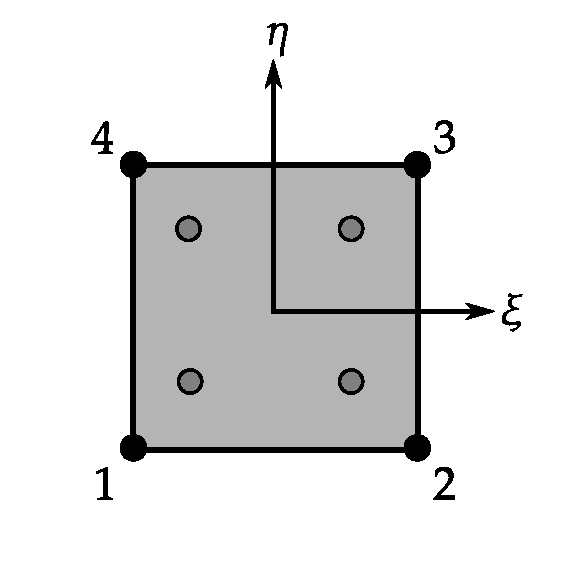
\includegraphics[width=0.3\textwidth]{figures/elements/quadrangle_4}
  \label{fig:elements:quadrangle4}
} & &
\subfloat[\code{quadrangle\_8}]{
  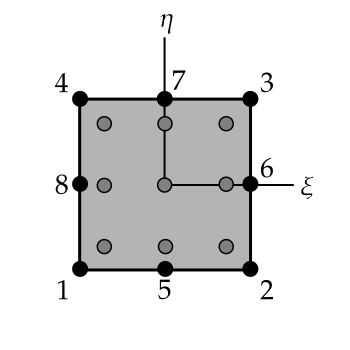
\includegraphics[width=0.3\textwidth]{figures/elements/quadrangle_8}
  \label{fig:elements:quadrangle8}
} 
\end{tabular}
\end{center}
\caption{A schematic overview of the four supported 2D element types in \akantu. In each element the node numbering as used in \akantu is indicated and also the quadrature points are highlighted (gray circles).}
\label{fig:elements:2D}
\end{figure}

\begin{table}[!htb]
\begin{center}
\begin{tabular}{l||c|c|c}
Element type & Order & \# nodes & \# quad. points \\
\hline
\code{triangle\_3} & linear & 3 & 1 \\
\code{triangle\_6} & quadratic & 6 & 3 \\
\hline
\code{quadrangle\_4} & quadratic & 4 & 4 \\
\code{quadrangle\_8} & cubic & 8 & 9 \\
\end{tabular}
\end{center}
\caption{Some basic properties of the four 2D isoparametric elements in \akantu.}
\label{tab:elements:2D}
\end{table}

%%%%%%%%%% 3D %%%%%%%%%
\subsection{Isoparametric Elements in 3D\index{Elements!3D}}

In \akantu there are three types of isoparametric elements defined in 3D. These element types are called \code{tetrahedron\_4}, \code{tetrahedron\_10} and \code{hexahedron\_8} and all of them are depicted schematically in Figure~\ref{fig:elements:3D}. As with the 1D and 2D elements some of the most basic properties of these elements are listed in Table~\ref{tab:elements:3D}.

\begin{figure}[!htb]
\begin{center}
\begin{tabular}{m{0.3\textwidth}m{0.3\textwidth}m{0.3\textwidth}}
\subfloat[\code{tetrahedron\_4}]{
  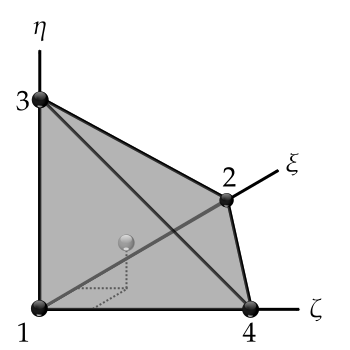
\includegraphics[width=0.3\textwidth]{figures/elements/tetrahedron_4}
  \label{fig:elements:tetrahedron4}
} &
\subfloat[\code{tetrahedron\_10}]{
  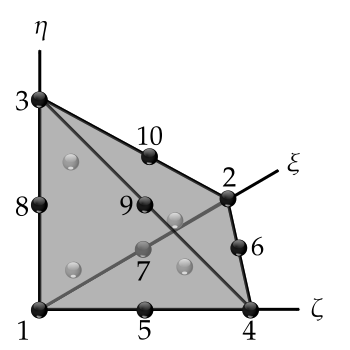
\includegraphics[width=0.3\textwidth]{figures/elements/tetrahedron_10}
  \label{fig:elements:tetrahedron10}
} &
\subfloat[\code{hexahedron\_8}]{
  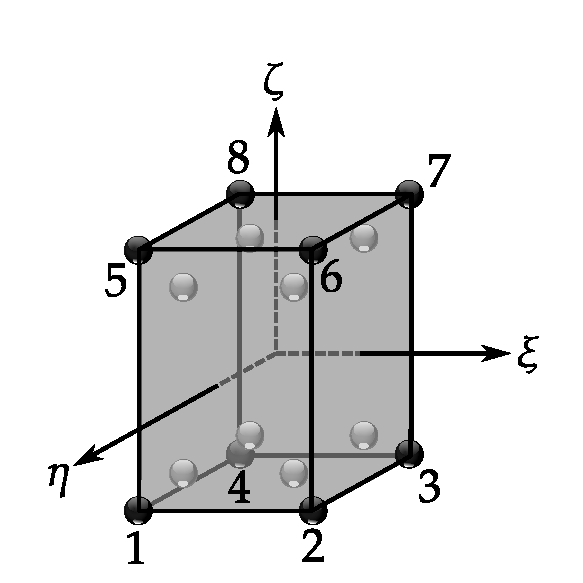
\includegraphics[width=0.3\textwidth]{figures/elements/hexahedron_8}
  \label{fig:elements:hexahedron8}
} 
\end{tabular}
\caption{A schematic overview of the three supported 3D element types in \akantu. In each element the node numbering as used in \akantu is indicated and also the quadrature points are highlighted (gray spheres).}
\label{fig:elements:3D}
\end{center}
\end{figure}

\begin{table}[!htb]
\begin{center}
\begin{tabular}{l||c|c|c}
Element type & Order & \# nodes & \# quad. points  \\
\hline
\code{tetrahedron\_4} & linear & 4 & 1  \\
\code{tetrahedron\_10} & quadratic & 10 & 4  \\
\hline
\code{hexahedron\_8} & cubic & 8 & 8  \\
\end{tabular}
\end{center}
\caption{Some basic properties of the three 3D isoparametric elements in \akantu.}
\label{tab:elements:3D}
\end{table}
